\documentclass[12pt, a4paper, oneside]{ctexart}
\usepackage{amsmath, amsthm, amssymb, graphicx}
\usepackage[bookmarks=true, colorlinks, citecolor=blue, linkcolor=black]{hyperref}
\usepackage[margin = 25mm]{geometry}
\usepackage{setspace}
\usepackage{listings}
\usepackage{cite}
\usepackage{xcolor}
\usepackage{float}

\definecolor{codegreen}{rgb}{0,0.6,0}
\definecolor{codegray}{rgb}{0.5,0.5,0.5}
\definecolor{codepurple}{rgb}{0.58,0,0.82}
\definecolor{backcolour}{rgb}{0.95,0.95,0.92}

\lstdefinestyle{mystyle}{
    backgroundcolor=\color{backcolour},   
    commentstyle=\color{codegreen},
    keywordstyle=\color{magenta},
    numberstyle=\tiny\color{codegray},
    stringstyle=\color{codepurple},
    basicstyle=\ttfamily\footnotesize,
    breakatwhitespace=false,         
    breaklines=true,                 
    captionpos=b,                    
    keepspaces=true,                 
    numbers=left,                    
    numbersep=5pt,                  
    showspaces=false,                
    showstringspaces=false,
    showtabs=false,                  
    tabsize=2
}

\lstset{style=mystyle}


\title{Use the Newton-Raphson method to solve non-linear equations}
\date{\today}
\author{phys.2001 孙陶庵 202011010101 }
\begin{document}
\begin{spacing}{2.0}
\tableofcontents
\maketitle
\section{Newton-Raphson method}
\subsection{code}
\begin{lstlisting}[language=Matlab, caption=Newton-Raphson method]
    clear
    x0 = [0.1,0.1,-0.1];
    eps = 1e-5;
    maxiter = 10;
    F = @(x)([3*x(1) - cos(x(2)*x(3)) - 1/2;
        x(1)^2 - 81*(x(2) + 0.1)^2 + sin(x(3)) + 1.06;
        exp(-x(1)*x(2)) + 20*x(3) + (10*pi - 3)/3]);
    J = @(x)([3 -x(3)*sin(x(2)*x(3)) -x(2)*sin(x(2)*x(3)); 
        2*x(1) -162*(x(2) + 0.1) cos(x(3));
        -x(2)*exp(-x(1)*x(2)) -x(1)*exp(-x(1)*x(2)) 20]);
    x = double(x0);
    for i = 1:maxiter
        Jx = J(x);
        Fx = F(x);
        delta = - Jx \ Fx;
        x = x + delta;
        if norm(delta) < eps
            return;
        end
    end
    x


if i == maxiter
    error('This method can''t execute');
end

    \end{lstlisting}
\subsection{Principle explanation\cite{key2}\cite{key3}}
Before we get to the code, we need to know how the method works. The Newton-Raphson method is an approximate solution to equations over real numbers and real
complex number fields. This method uses the antecedent of the Taylor series of the function $f(x)$ to find the roots
The equation $f(x)=0$. \\
First choose a $x_0$ close to the zero of the function $f(x)$ and compute the corresponding $f(x_0)$
and the slope of the tangent line $f'(x_0)$ (where $f'$ represents the derivative of the function $f$).
Then we calculate the intersection of the line through the points $(x_0, f(x_0))$ and $f'(x_0)$
axis and the $x$-coordinate of the $x$-axis, which is the solution of the following equation.
\begin{center}
    $0= (x-x_0)\cdot f'(x_0)+f(x_0)$
\end{center}

We name the newly obtained $x$ coordinates of the point as $x_1$.
Usually, $x_1$ is closer to the solution of the equation $f(x)=0$ than $x_0$.
So we can now start the next iteration from $x_1$. The iteration equation can be simplified to:
\begin{center}
    $x_{n+1} = x_n - \frac{f(x_n)}{f'(x_n)}$
\end{center}

It has been proved that the quadratic convergence of the Newton iteration method must meet the following conditions: 
$f'(x) \ne 0$; For all $x\in I$, where $I$ is the 
interval $[\alpha - \gamma, \alpha + \gamma]$, and $x_0$ is in the interval $I$, 
namely $ r \geqslant \left| a-x_0 \right|$;
$f''(x)$ is continuous for all $x\in I$;$x_0$ is close enough to the root $\alpha$.
However, the method above is just a function solver. If we want to get the algorithm for nonlinear 'equations' like follow:

\begin{center}
    $    \begin{cases}
            3x_{1} - \cos{(x_{2}x_{3})} - \frac{1}{2} = 0 \\
            x_{1}^{2} - 81(x_{2} + 0.1)^{2} + \sin(x_{3}) + 1.06 = 0 \\
            e^{-x_{1}x_{2}} + 20x_{3} + \frac{10\pi - 3}{3} = 0
        \end{cases} $       
\end{center}

Then we need to expand the definition from $f'(x_n)$ to $\nabla f(x)$. The equations' form will be changed as follow\cite{enwiki:1141352419}:
\begin{center}
    $\begin{bmatrix}
        \dfrac{\partial \mathbf{f}}{\partial x_1} & \cdots & \dfrac{\partial \mathbf{f}}{\partial x_n}
      \end{bmatrix}
      = \begin{bmatrix}
        \nabla^{\mathrm T} f_1 \\  
        \vdots \\
        \nabla^{\mathrm T} f_m   
      \end{bmatrix}
      = \begin{bmatrix}
          \dfrac{\partial f_1}{\partial x_1} & \cdots & \dfrac{\partial f_1}{\partial x_n}\\
          \vdots                             & \ddots & \vdots\\
          \dfrac{\partial f_m}{\partial x_1} & \cdots & \dfrac{\partial f_m}{\partial x_n}
      \end{bmatrix}$
\end{center}
This matrix are called Jacobian matrix. And we will get:
\begin{center}
    $x_{n+1} = x_n - J^{-1}(x_n)f'(x_n)$
\end{center}
\subsection{code-explanation}
We can see the code above. We use anonymous function to define 2 functions first, F is original function. 
The next "function" is Jacobi matrix:
\begin{center}
    $J(x) = \begin{pmatrix}
        3 & -x_{3}\sin{(x_{2}x_{3})} & -x_{2}\sin{(x_{2}x_{3})} \\
        2x_{1} & -162(x_{2} + 0.1)\cos(x_{3}) & -x_{1}\exp{(-x_{1}x_{2})} \\
        -x_{2}\exp{(-x_{1}x_{2})} & -x_{1}\exp{(-x_{1}x_{2})} & 20
        \end{pmatrix}
        $
\end{center}
Now, we can get the final result:
\begin{center}
$    \begin{pmatrix}
        0.5000 & 0.5000 & 0.3000 \\
        0.0000 & 0.0000 & -0.2000 \\
        -0.5236 & -0.5236 & -0.7236
        \end{pmatrix}
$        
\end{center}


\section{Gauss-Seidel method}

\begin{lstlisting}[language=Matlab, caption=Newton-Raphson method]
x = [0.1,0.1,-0.1];
eps = 1e-5;
err = 10;

while(err>eps)
    y = g(x);
    err = norm(y-x);
    x = y;
end

x

function y = g(x)
    y(1) = 1/3*cos(x(2)*x(3))+1/6;
    y(2) = 1/9*sqrt(x(1)^2+sin(x(3))+1.06)-0.1;
    y(3) = -exp(-x(1)*x(2))/20-(10*pi-3)/60;
end

\end{lstlisting}

The above code is derived from the class.


\section{Jacobian method}
I'm so sorry that I can't accurately understand the difference between Gauss-Seidel algorithm and Jacobi algorithm.
\section{Convergence speed for iterative methods}
The principle of convergence speed has been paid in the reference\cite{key1}, so I won't go into details here.
\subsection{Newton-Raphson method}
\begin{lstlisting}[language=Matlab, caption=Newton-Raphson method with Convergence speed for iterative methods] 
    clear
    x0 = [0.1,0.1,-0.1];
    eps = 1e-5;
    maxiter = 10;
    F = @(x)([3*x(1) - cos(x(2)*x(3)) - 1/2;
        x(1)^2 - 81*(x(2) + 0.1)^2 + sin(x(3)) + 1.06;
        exp(-x(1)*x(2)) + 20*x(3) + (10*pi - 3)/3]);
    J = @(x)([3 -x(3)*sin(x(2)*x(3)) -x(2)*sin(x(2)*x(3)); 
        2*x(1) -162*(x(2) + 0.1) cos(x(3));
        -x(2)*exp(-x(1)*x(2)) -x(1)*exp(-x(1)*x(2)) 20]);
    x = double(x0);
    alpha111 = zeros(1, maxiter);
    
    for i = 1:maxiter
        Jx = J(x);
        Fx = F(x);
        delta = - Jx \ Fx;
        x = x + delta;
        alpha111(i) = norm(Fx);
        if norm(delta) < eps
            break;
        end
    end
    semilogy(1:i, alpha111(1:i), 'o-');
    xlabel('Iteration');
    ylabel('alpha');    
\end{lstlisting}
\subsection{Gauss-Seidel method}
\begin{lstlisting}[caption=Gauss-Seidel method with Convergence speed for iterative methods] 
    x = [0.1,0.1,-0.1];
    eps = 1e-5;
    err = 10;
    order11 = [];
    
    while(err>eps)
        y = g(x);
        err = norm(y-x);
        order11 = [order11 err];
        x = y;
    end
    
    p = polyfit(log(order11(1:end-1)), log(order11(2:end)), 1);
    convergence_rate = p(1);
    
    semilogy(order11);
    title(['Convergence rate: ', num2str(convergence_rate)]);
    xlabel('Iteration');
    ylabel('Error');
    
    
    function y = g(x)
        y(1) = 1/3*cos(x(2)*x(3))+1/6;
        y(2) = 1/9*sqrt(x(1)^2+sin(x(3))+1.06)-0.1;
        y(3) = -exp(-x(1)*x(2))/20-(10*pi-3)/60;
    end
    

\end{lstlisting}
\subsection{Jacobi method}
\section{Convergence Rate Comparison of Different Algorithms}
\begin{figure}[H]
	\centering
	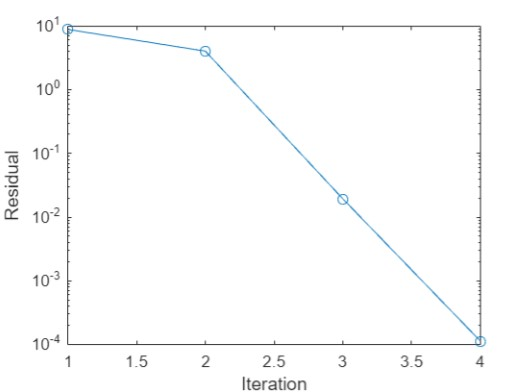
\includegraphics[width=8cm]{newtonlaw.jpg}
	\caption{newtonlaw}
\end{figure}
\begin{figure}[H]
	\centering
	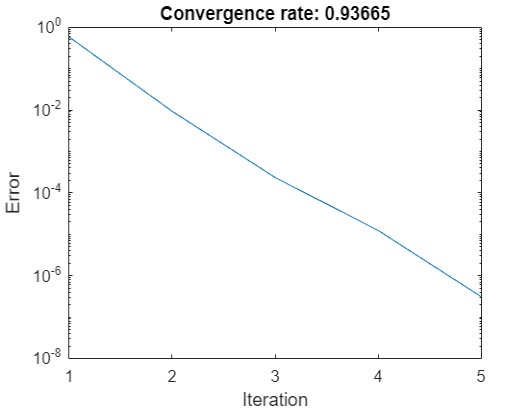
\includegraphics[width=8cm]{Gauss.jpg}
	\caption{Gauss}
\end{figure}

\end{spacing}{}

\bibliographystyle{IEEEtran}
\bibliography{alpha1}

\end{document}